\documentclass{article}
\usepackage[english]{babel}
\usepackage[letterpaper,top=2cm,bottom=2cm,left=2.5cm,right=2.5cm,marginparwidth=1.25cm]{geometry}

\usepackage{hyperref, booktabs, float}
\usepackage[leqno]{amsmath}
\usepackage{enumitem, nccmath,lipsum,amssymb,xcolor,xparse,listings, blindtext}
\usepackage[most]{tcolorbox}

\usepackage{graphicx}
\graphicspath{ {./attachments/} }

\NewDocumentCommand{\codeword}{v}{\texttt{\textcolor{blue}{#1}}}

\lstset{language=C, keywordstyle={\bfseries \color{blue}}}

\NewDocumentCommand{\mynote}{+O{}+m}{%
  \begingroup
  \tcbset{%
    noteshift/.store in=\mynote@shift,
    noteshift=1.5cm
  }
  \begin{tcolorbox}[nobeforeafter,
    enhanced,
    sharp corners,
    toprule=0.5pt,
    bottomrule=0.5pt,
    leftrule=0pt,
    rightrule=0pt,
    colback=green!10,
    #1,
    left skip=\mynote@shift,
    right skip=\mynote@shift,
    overlay={\node[right] (mynotenode) at ([xshift=-\mynote@shift]frame.west) {\textbf{Note:}} ;},
    ]
    #2
  \end{tcolorbox}
  \endgroup
  }
\makeatother

\newcommand{\mytext}[1]% #1 = same as intertext
{&\parbox{0.9\textwidth}{\rule{0pt}{.5\baselineskip}\\
\textrm{#1}\\
\rule{0pt}{.5\baselineskip}}&\\}

\newcounter{exercise}
\newcounter{problem}[exercise]
\newcommand{\myitem}{\stepcounter{problem}\tag*{\alph{problem})}}

\title{Lab 4: Bash scripting}
\author{Mashenkov Timofei B23-CBS-02 \\ \href{mailto:t.mashenkov@innopolis.university}{t.mashenkov@innopolis.university}}
\begin{document}
\maketitle{}

\section{User and System Details}
\noindent

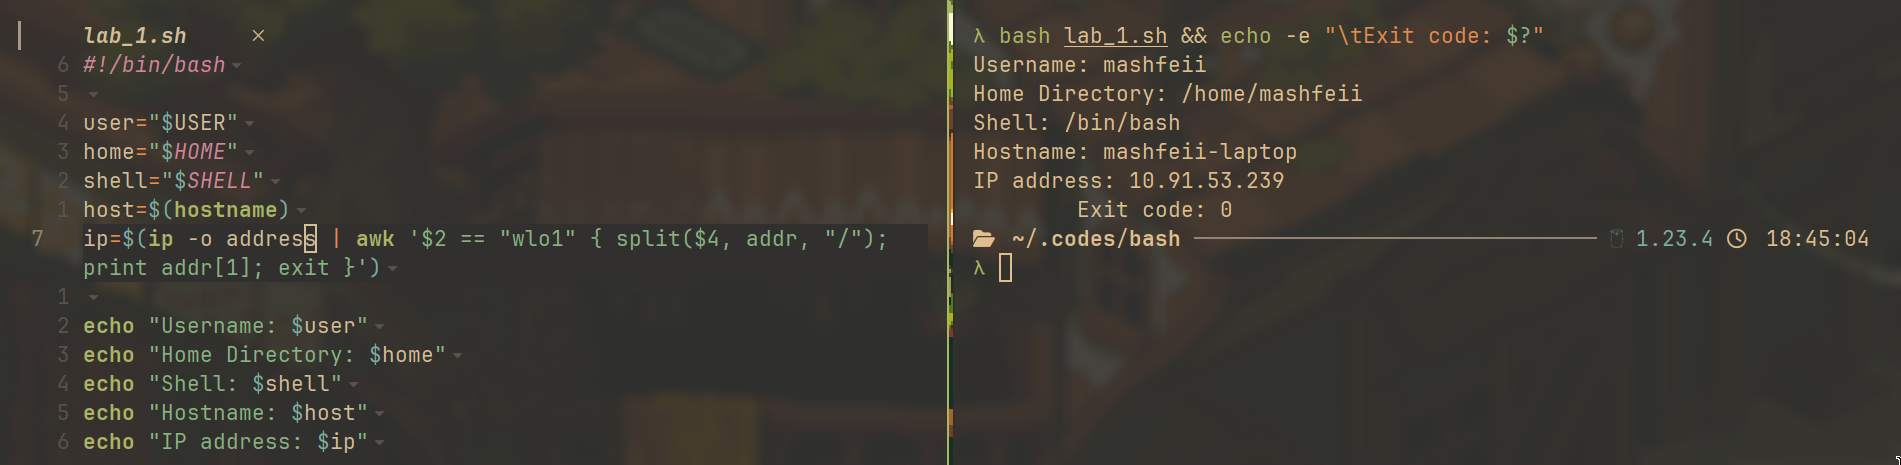
\includegraphics[width=460pt]{4_1.jpg}
\newline

The script is a sequential output of system variables, so it does not require in-depth testing, a possible error may
occur if the \codeword{ip} command is missing (for example, the \codeword{ifconfig} command is missing in my system)

\section{Home Directory Backup}
\noindent

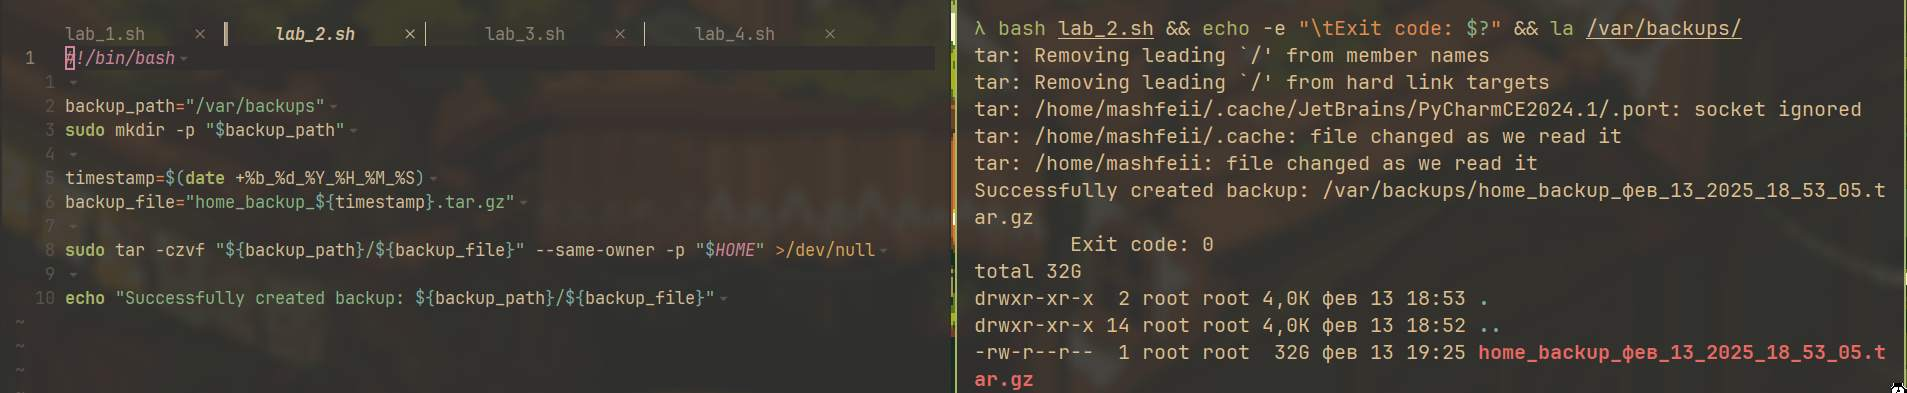
\includegraphics[width=460pt]{4_2.jpg}
\newline

In this script, after testing, it was possible to find the absence of \codeword{sudo} in key places, no errors were
detected during the compression of the home folder, although the process took a long time. \\
The \codeword{--same-owner} and \codeword{--same-permissions} flags were used to fulfill the task requirements. \\
The file name is slightly different from the example in the assignment due to the global language of the system, but the format is identical.

\section{System Artifacts}
\noindent

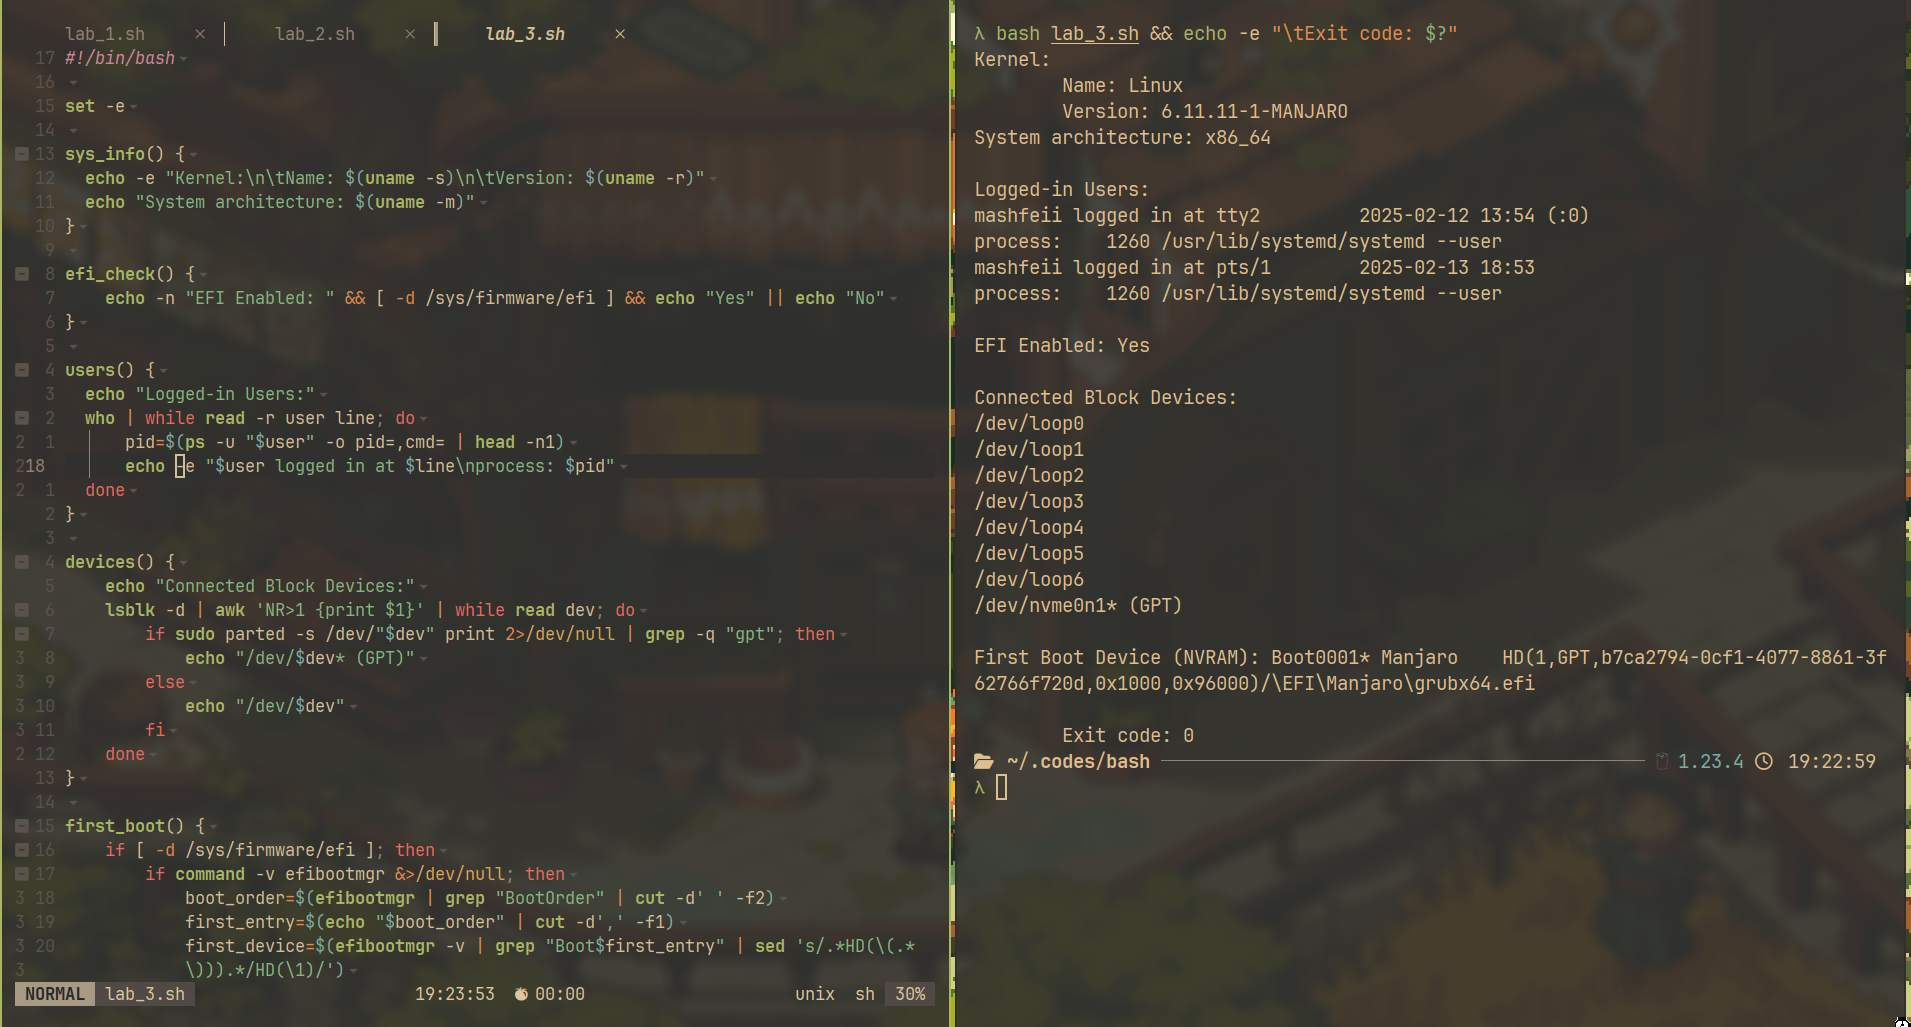
\includegraphics[width=460pt]{4_3.jpg}
\newline

This script uses the \codeword{set -e} construct to exit the script early in case of any function error exit code.

\section{Bonus}
\noindent

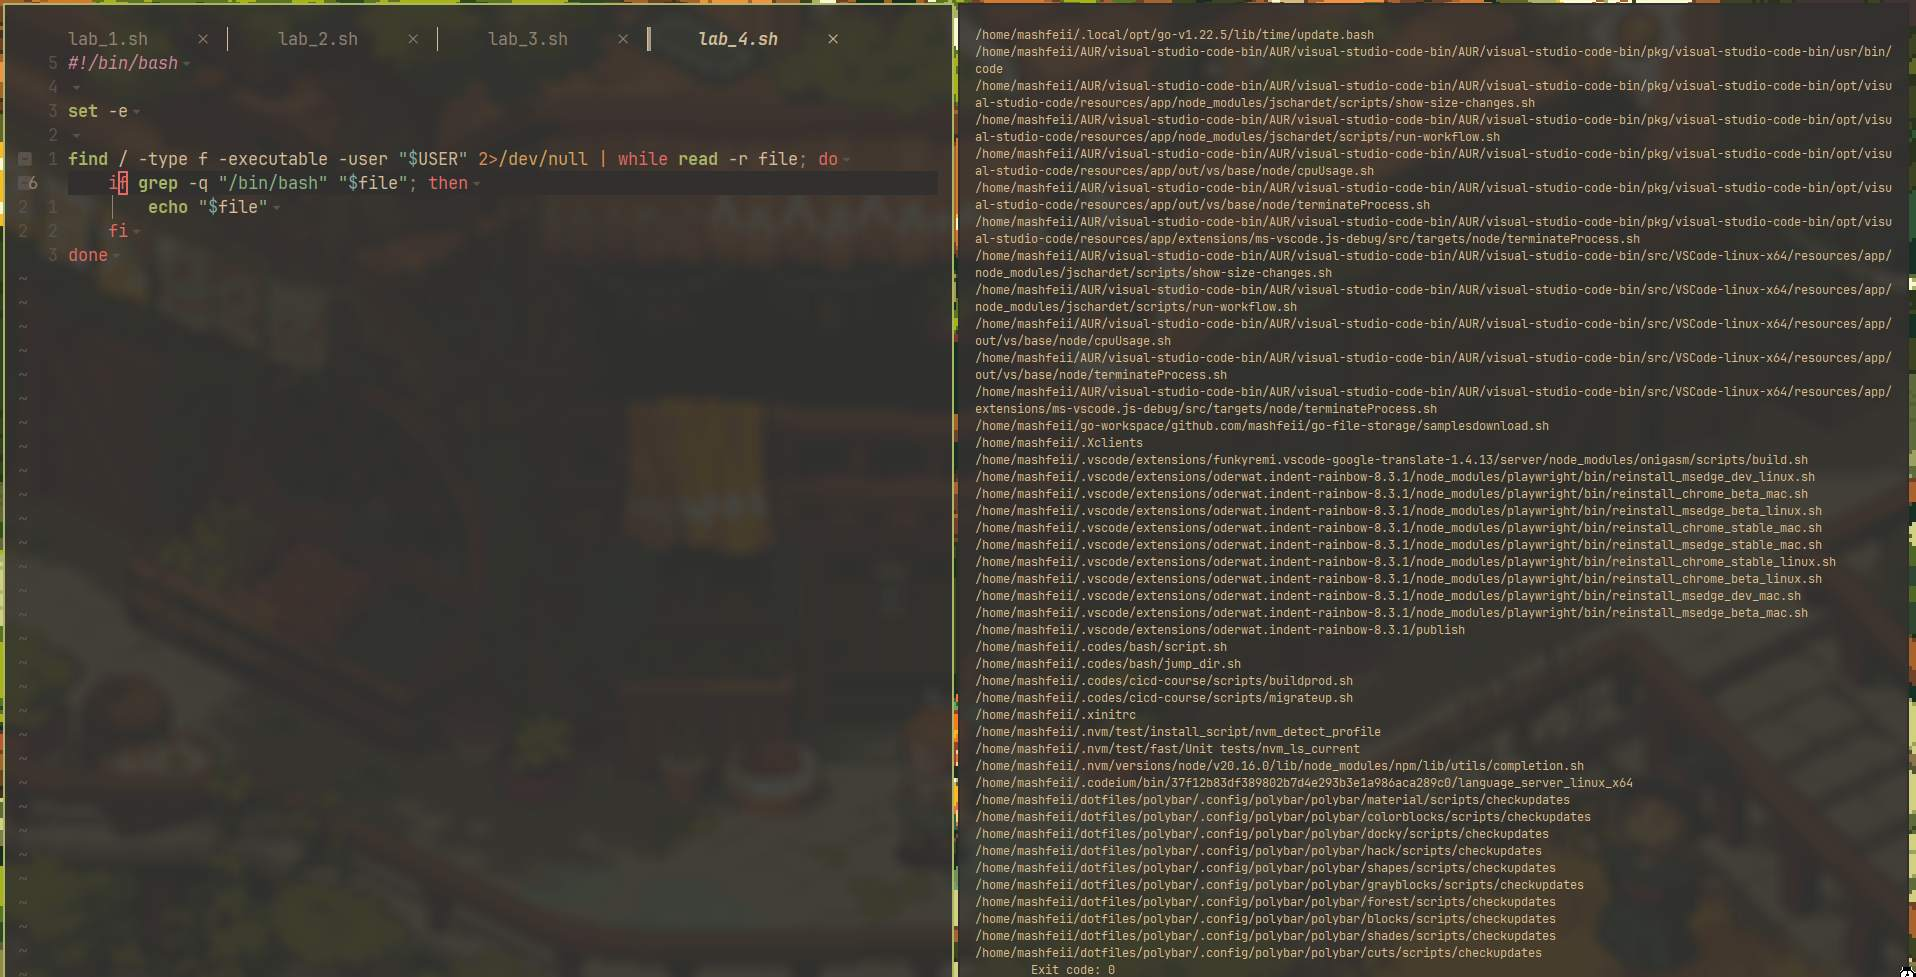
\includegraphics[width=460pt]{4_4.jpg}
\newline

First, using the \codeword{find} command, I find all the files I am interested in, fulfilling the conditions of the task, then, reading each file, I try to find the line of interest, exiting the search immediately after the first match.

\end{document}
